%auteur: Amaury JOLY
\begin{frame} 
  \frametitle{Qu’est-ce qu’un relay ?} 
  \begin{itemize} 
    \item Une Application décentralisée jouant le rôle de: 
    \begin{itemize}
      \item suiveur d’état de chaînes connectées.
      \item transmetteur d’informations entre blockchains.
      \item prouveur de transactions cross-chain.
    \end{itemize}
  \end{itemize} 
\end{frame}

\begin{frame}
  \frametitle{Qu’est-ce que BTCRelay ?}
  \begin{figure}
    \centering
    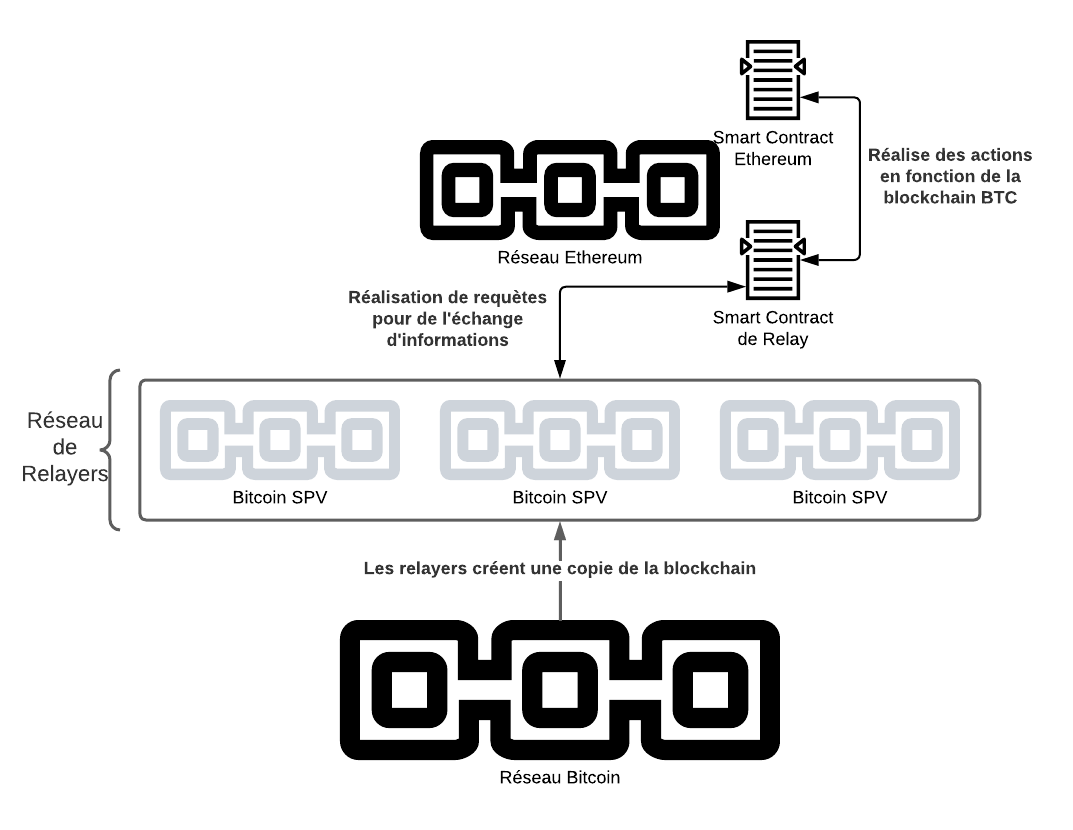
\includegraphics[scale = 0.22]{decentralisation/btcRelay.png}
    \caption{BTCRelay}
  \end{figure}
\end{frame}


\begin{frame}
  \frametitle{Qu’est-ce que tBTC ?}
  \begin{figure}
    \centering
    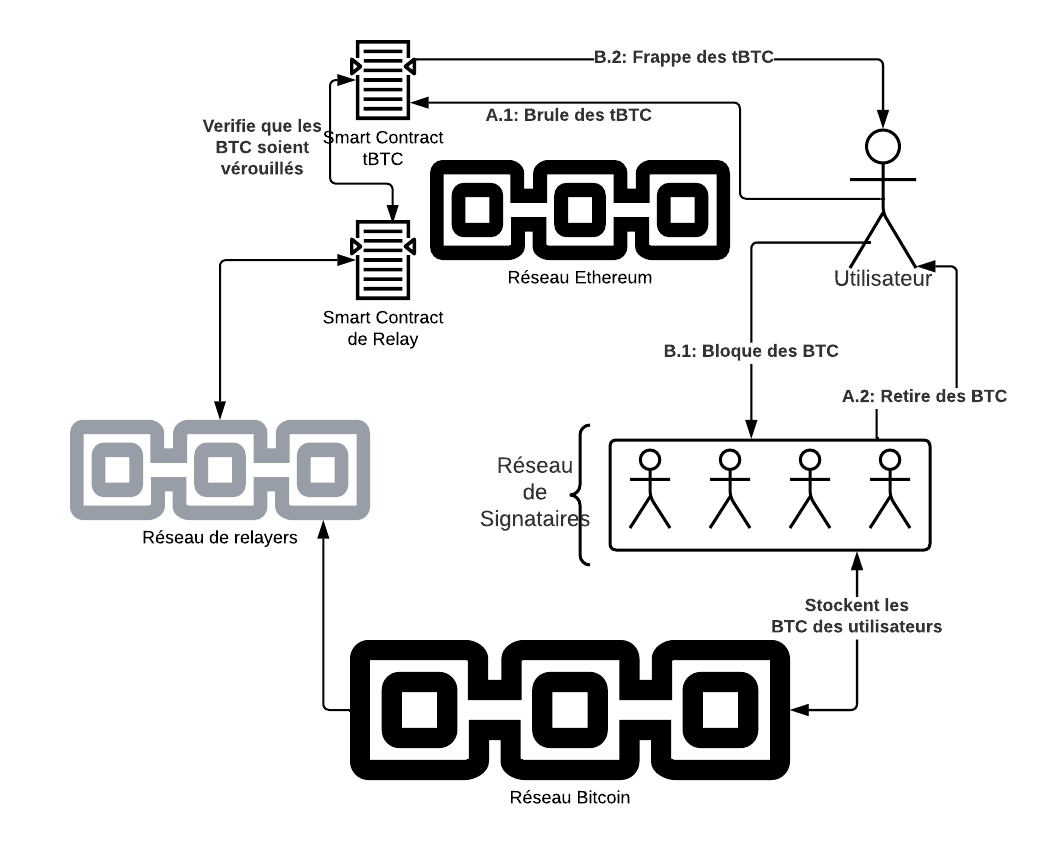
\includegraphics[scale = 0.22]{decentralisation/tBTC.png}
    \caption{tBTC}
  \end{figure}
\end{frame}

\begin{frame}
  \frametitle{Limitations des relays}
  \begin{itemize}
    \item Avantages:
    \begin{itemize}
      \item N'importe qui peut participer aux réseaux.
      \item Peu de risques pour l'utilisateur.
    \end{itemize}
    \item Désavantages:
    \begin{itemize}
      \item Disponibilité du service dépendant des signataires.
      \item Réseau de relayers sur du PoS.
      \begin{itemize}
        \item Si le réseau est trop petit, le coût pour une attaque 51\% est faible.
      \end{itemize}
    \end{itemize}  
  \end{itemize}
\end{frame}